\documentclass{article}

\usepackage[final]{pdfpages}
\setboolean{@twoside}{false}
\usepackage{hyperref}
\usepackage[toc,page]{appendix}
\usepackage{tikz}
\usepackage{graphicx}
\usepackage{caption}
\usepackage{subcaption}
\usepackage{amsmath}
\usepackage[letterpaper, top=1in, bottom=1in, left=1in, right=1in]{geometry}
\usepackage{listings}
\usepackage{color}
\definecolor{mygreen}{RGB}{28,172,0} % color values Red, Green, Blue
\definecolor{mylilas}{RGB}{170,55,241}
\lstset{language=Matlab,%
    basicstyle=\footnotesize,
    breaklines=true,%
    morekeywords={matlab2tikz},
    keywordstyle=\color{blue},%
    morekeywords=[2]{1}, keywordstyle=[2]{\color{black}},
    identifierstyle=\color{black},%
    stringstyle=\color{mylilas},
    commentstyle=\color{mygreen},%
    showstringspaces=false,%without this there will be a symbol in the places where there is a space
    numbers=left,%
    numberstyle={\tiny \color{black}},% size of the numbers
    numbersep=9pt, % this defines how far the numbers are from the text
    emph=[1]{for,end,break},emphstyle=[1]\color{red}, %some words to emphasise
}

\title{ECSE 493 --- Controls\&Robotics Lab\\Lab 23 Report}
\author{\textbf{David Lavoie-Boutin} 260583602\\ \textbf{Jake Macneal}, 260566105}

\date{\today}

\begin{document}

\maketitle
\section*{Part 1}
\subsection*{1}
Starting from the results of lab 2, we know that the critically damped response will be achieved with a proportional gain higher than 20 and lower than 100. By trial and error, following a binary search approach, we can determine a best gain $K_p = 40$. This is the maximal gain we can use without creating too much overshoot. With the experimental setup, we achieve the following response:

\begin{figure}[!htb]
\centering
\includegraphics[width=0.7\textwidth]{crit_damped.eps}
\end{figure}

This response has a maximum overshoot of 0.0027 meters and a steady-state error of 1.5512\%.
\clearpage
\subsection*{2}
In lab 2, we determined the experimental transfer function of the cart system to be: $G(s) = \frac{1}{14.62+1.49s}$. Considering the closed loop equation with a proportional gain controller, we can derive the system equation as follow:
\begin{eqnarray*}
    \frac{Y}{X} &=& \frac{H(s)G(s)}{1+H(s)G(s)}\\
    &=&\frac{K_p*\frac{1}{14.62+1.49s}}{1+K_p*\frac{1}{14.62+1.49s}}\\
    &=& \frac{1}{14.62+1.49s + K_p}
\end{eqnarray*}

Now let $K_p = 40$ and we get $\frac{1}{54.62+1.49s}$
\subsection*{3}
We modified the Simulink diagram by adding a derivative operator and a summation block as shown in the following figure:
\begin{figure}[!htb]
\centering
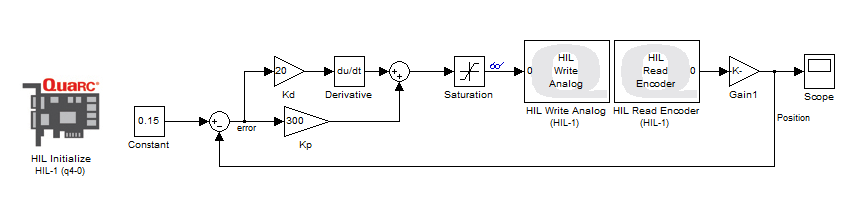
\includegraphics[width=\textwidth]{lab3_pd.PNG}
\end{figure}

Using this schematic, we performed several simulations gradually increasing the value of $K_d$. These are the results we came up with.

\begin{figure}[!htb]
\centering
\includegraphics[width=0.7\textwidth]{effect_kd.eps}
\end{figure}

On the step responses, we can see that increasing the differential gain causes several things to happen. First, the rise time is increased and smoothen out the deceleration when reaching the steady state; we also see that the steady state error increases. Finally, we completely eliminate the already very small overshoot.

\subsection*{4}

To tune our system, we started with tuning the proportional gain alone. We increased it quite a significant amount to achieve a super fast rise time. Since we saturate the input of the plant to 5V, past $K_p = 300$ we do not see much improvement in the rise time but we do increase the overshoot. After that, we increased the gain of the differential term until we eliminate the overshoot, this happens around $K_d = 20$ and yields the following response with no overshoot and a 0.34 second rise-time:

\begin{figure}[!htb]
\centering
\includegraphics[width=0.7\textwidth]{pd_ctrl.eps}
\end{figure}

\subsection*{5}

\end{document}